
\chapter{An intrinsic notion of rank for factor models}

As Moore's Law progresses, data sets measuring on the order of hundreds or
thousands of variables are becoming increasingly more common. Making sense of
data of this size is simply not tractable without imposing a simplifying
model. One popular simplification is to posit existence of a small number of
common factors that drive the dynamics of the data, which are usually
estimated by principal components analysis (PCA) or some variation thereof.
The $n \times p$ data matrix $\mX$ is approximated as a low-rank product $\mX
\approx \mU \mV^\trans$, where $\mU$ and $\mV$ are $n \times k$ and $p \times
k$, respectively, with $k$ much smaller than $n$ and $p$.

The number of algorithms for approximating matrices by low-rank products has
exploded in recent years. These algorithms include archetypal analysis
\cite{cutler1994aa}, the semi-discrete decomposition (SDD)
\cite{kolda1998smd}, the non-negative matrix factorization (NMF)
\cite{lee1999lpo}, the plaid model \cite{lazzeroni2002pmg}, the $CUR$
decomposition \cite{drineas2007fmc}, and regularized versions thereof. They
also include some clustering methods, in particular $k$-means and fuzzy
$k$-means \cite{bezdek1980fmp}.

A prevailing question is: How many common factors underly a data set? In other
words, how should one choose $k$? In general, the answer to this question is
application-specific. If we are trying to use $\mX$ to predict a response,
$y$, then the optimal $k$ is the one that gives the best prediction error
for $y$. The situation is not always this simple, though. For exploratory
analysis, there is no external response, and we want to choose a $k$ that is
``intrinsic'' to $\mX$. For other applications, we don't have a single
response, $y$, we have \emph{many} responses $y_1, y_2, \ldots, y_m$.
We may not even know all of the $y_i$ when we are processing $\mX$. We want a $k$ that has good average-case or worst-case prediction properties for a large class of responses.

In this chapter, we develop a precise notion of intrinsic rank for ``latent
factor'' matrix data. This choice of $k$ is the one that minimizes average- or
worst-case prediction error over all bilinear statistics. We specifically work
with the singular value decomposition (SVD), but our definition can be
extended to other matrix factorizations as well.

Section~\ref{S:latent-factor-model} introduces the latent factor model, the
data model from which we base our constructions.
Section~\ref{S:intrinsic-rank} defines intrinsic rank as the minimizer of a
loss function. We give a theoretical analysis of the behavior of some natural
loss functions in Section~\ref{S:loss-behavior}, followed by simulations in
Section~\ref{S:intrinsic-loss-simulations}. In
Section~\ref{S:intrinsic-rank-scree-plot}, we examine the connection between
intrinsic rank and the scree plot. Finally,
Section~\ref{S:intrinsic-rank-extensions} discusses some extensions.


\section{The latent factor model}\label{S:latent-factor-model}

We start by describing a model for data generated by a small number of latent
factors and additive noise. Suppose that we have $n$ multivariate observations
$\vx_{1}, \vx_{2}, \ldots, \vx_{n} \in \reals^p$. In a microarray setting, we
will have about $n=50$ arrays measuring the activations of around $p=5000$
genes. Alternatively, for financial applications $\vx_i$ will measure the
market value of on the order of $p=1000$ assets on day $i$, and we may be looking at
data from the last three years, so $n \approx 1000$. In these situations and
others like them, we can often convince ourselves that there aren't really
$5000$ or $1000$ different things going on in the data. Probably, there are a small number, $k$ of unobserved factors driving the dynamics of the data. Typically, in fact, we think $k$ is on the order of around $5$ or $10$.

To be specific about this intuition, for genomics applications, we don't
really think that all $p=5000$ measured genes are behaving independently. On
the contrary, we think that there are a small number of biological processes
that determine how much of each protein gets produced. In finance, while it is
true that the stock prices of individual companies have a certain degree of
independence, often macroscopic effects like industry- and market-wide trends
can explain a substantial portion of the value.

\subsection{The spiked model}

One way to model latent effects is to assume that the $\vx_i$ are \iid and
that their covariance is ``spiked''. We think that $\vx_i$ is a weighted
combination of $k$ latent factors corrupted by additive white noise. In this
case, $\vx_i$ can be decomposed as
\begin{align}
    \vx_i
        &=
        \sum_{j=1}^k
            \va_j
            s_{i,j}
        +
        \vepsilon_i \notag \\
        &=
        \mA \vs_i + \vepsilon_i,
\end{align}
where
\(
    \mA
    =
    \left(
    \begin{matrix}
        \va_1 & \va_2 & \cdots & \va_k
    \end{matrix}
    \right)
\)
is a $p \times k$ matrix of latent factors common to all observations and
$\vs_i \in \reals^{k}$ is a vector of loadings for the $i$th observation. We assume that the
noise vector $\vepsilon_i$ is distributed as $\Normal( 0, \, \sigma^2 \mI_p
)$. If the loadings have mean zero and covariance $\mSigma_\text{S} \in
\reals^{k \times k}$, and if they are also independent of the noise, then
$\vx_i$ has covariance
\begin{equation}\label{E:spiked-cov-natural-form}
    \mSigma
        \define
        \E \left[ \vx_i \, \vx_i^\trans \right]
            =
                \mA \mSigma_\text{S} \mA^\trans
                +
                \sigma^2
                \mI_p.
\end{equation}
The decomposition in \eqref{E:spiked-cov-natural-form} can be reparametrized
as
\begin{equation}\label{E:spiked-cov-identifiable-form}
    \mSigma
        =
        \mQ \mLambda \mQ^\trans
        +
        \sigma^2
        \mI_p,
\end{equation}
where $\mQ^\trans \mQ = \mI_k$ and
\(
    \mLambda
        = 
        \diag \left( \lambda_1, \lambda_2, \ldots, \lambda_k \right),
\)
with $\lambda_1 \geq \lambda_2 \geq \cdots \geq \lambda_k \geq 0$.
Equation~\eqref{E:spiked-cov-identifiable-form} makes it apparent that
$\mSigma$ is ``spiked'', in the sense that most of its eigenvalues are equal,
but $k$ eigenvalues stand out above the bulk. The first $k$ eigenvalues are
$\lambda_1 + \sigma^2, \lambda_2 + \sigma^2, \ldots, \lambda_k + \sigma^2$,
and the remaining $p-k$ eigenvalues are equal to $\sigma^2$.

\subsection{More general matrix models}

We can introduce a model more general than the spiked one by specifying
a distribution for the $n\times p$ data matrix 
\(
    \mX
    =
    \left(
    \begin{matrix}
        \vx_1 &
        \vx_2 &
        \cdots &
        \vx_n
    \end{matrix}
    \right)^\trans
\)
that includes dependence between the rows.  In the spiked model, the
distribution of $\mX$ can be described as
\begin{equation}\label{E:data-matrix-spiked}
    \mX
        \eqd
        \mZ
        \mLambda^{1/2}
        \mQ^\trans
        +
        \mE,
\end{equation}
where 
\(
    \mE 
        = 
        \left(
        \begin{matrix}
            \vepsilon_1 & \vepsilon_2 & \cdots \vepsilon_n
        \end{matrix}
        \right)^\trans
\)
and $\mZ$ is an $n \times k$ matrix of independent 
$\Normal \left( 0, \, 1 \right)$ elements.  More generally, we can consider
data of the form
\begin{equation}\label{E:data-matrix-general}
    \mX
        \eqd
            \sqrt{n} \,
            \mU
            \mD
            \mV^\trans
            +
            \mE,
\end{equation}
where $\mU^\trans \mU = \mV^\trans \mV = \mI_k$, and $\mD = \diag( d_1, d_2,
\ldots, d_k )$ with $d_1 \geq d_2 \geq \cdots \geq d_k \geq 0$. We can get
\eqref{E:data-matrix-general} from \eqref{E:data-matrix-spiked} by letting
$\mZ \mLambda^{1/2} = \sqrt{n} \, \mU \mD \mC^\trans$ be the SVD of $\mZ
\mLambda^{1/2}$ and defining $\mV = \mQ \mC$. Unlike the spiked model,
\eqref{E:data-matrix-general} can model dependence between variables as well
as dependence between observations.

\section{An intrinsic notion of rank}\label{S:intrinsic-rank}

With Section~\ref{S:latent-factor-model}'s latent factor model in mind, we
turn our attention to defining the intrinsic rank of a data set. This
definition will be motivated both by the generative model for $\mX$ and by
predictive power considerations.  When 
\(
    \mX = \sqrt{n} \, \mU \mD \mV^\trans + \mE,
\)
we think of $\sqrt{n} \, \mU \mD \mV^\trans$ as ``signal'' and $\mE$ as ``noise''.  We make a distinction between the generative rank and the effective rank.

\begin{definition}
    If the $n \times p$ matrix $\mX$ is distributed as
    \(
        \mX = \sqrt{n} \, \mU \mD \mV^\trans + \mE,
    \)
    where $\mU^\trans \mU = \mV^\trans \mV = \mI_{k_0}$, $\mD$ is a
    $k_0 \times k_0$ diagonal matrix with positive diagonal entries, and $\mE$
    is a noise matrix independent of the signal term whose elements are
    \iid $\Normal( 0, \, \sigma^2 )$, then
    we denote by $k_0$ the \emph{generative rank} of $\mX$.
\end{definition}

\noindent 
Intuitively the generative rank is the rank of the signal part of $\mX$.

The effective rank is defined in terms of how well the first terms of the
SVD of $\mX$ approximates the signal $\sqrt{n} \, \mU \mD \mV^\trans$.  We
let $\mX = \sqrt{n} \mhU \mhD \mhV^\trans$ be the full SVD of $\mX$, where
\(
    \mhU
    =
    \left(
    \begin{matrix}
        \vhu_1 & \vhu_2 & \cdots & \vhu_{n\wedge p}
    \end{matrix}
    \right),
\)
\(
    \mhV
    =
    \left(
    \begin{matrix}
        \vhv_1 & \vhv_2 & \cdots & \vhv_{n\wedge p}
    \end{matrix}
    \right),
\)
and
\(
    \mhD
    =
    \diag \left(
        \hd_1, \hd_2, \ldots, \hd_{n\wedge p}
    \right).
\)
If we let
\(
    \mhD(k)
    =
    \diag \left(
        \hd_1, \hd_2, \ldots, \hd_k, 0, 0, \ldots, 0
    \right),
\)
then the SVD truncated to $k$ terms is
\(
    \mhX(k)
    =
    \sqrt{n} \,
    \mhU \mhD(k) \mhV^\trans.
\)
We are now in a position to define effective rank

\begin{definition}
    Given a loss function
    \(
        L : \reals^{n \times p} \times \reals^{n \times p} \to \reals,
    \)
    the effective rank of $\mX$ with respect to $L$ is equal to
    \[
        k_L^\ast
        \define
        \argmin_k \, 
            L \left( 
                \sqrt{n} \mU \mD \mV^\trans\!, \, \mhX(k) 
            \right).
    \]
\end{definition}

The effective rank depends on the choice of loss function.  In some settings it is preferable to choose an application-specific loss function.  Often, we appeal to simplicity and convenience and choose squared Frobenius loss.  Specifically,
\[
    L_\Frob ( \mA, \, \mA' )
        = \| \mA - \mA' \|_\Frob^2.
\]
One way to motivate this loss function is that it measures average squared error over all bilinear statistics of the form 
$\valpha^\trans \mA \, \vbeta$,
\[
    \frac{1}{np} \,
    \| \mA - \mA' \|_\Frob^2
    =
    \int\limits_{ \substack{ \| \valpha \|_2 = 1, \\
                             \| \vbeta \|_2  = 1 } }
        \!\!\!\!
        \left(
            \valpha^\trans \mA \, \vbeta
            -
            \valpha^\trans \mA' \vbeta
        \right)^2
        d\valpha \,
        d\vbeta
\]
(see Section~\ref{S:probabilistic-frob} for details).
In the context of the latent factor model, the effective rank with respect
to $L_\Frob$ is the rank that gives the best average-case predictions of 
bilinear statistics of the signal part (with respect to squared-error loss). 

A common alternative to Frobenius loss is spectral loss, given by
\[
    L_2 ( \mA, \, \mA' )
        = \| \mA - \mA' \|_2^2.
\]
This can be interpreted as worst-case squared error over the class of all 
bilinear statistics,
\[
    \| \mA - \mA' \|_2^2
        =
            \sup_{ \substack{ \| \valpha \|_2 = 1, \\
                              \| \vbeta \|_2  = 1 } }
                \left(
                    \valpha^\trans \mA \, \vbeta
                    -
                    \valpha^\trans \mA' \vbeta
                \right)^2.
\]
In the sequel, we denote the optimal ranks with respect to Frobenius and
spectral loss as $k^\ast_\Frob$ and $k^\ast_2$, respectively.


\section{Loss behavior}\label{S:loss-behavior}

In this section we investigate the behavior of the loss functions introduced
in Section~\ref{S:intrinsic-rank}.  First, we need to be more precise about
our working assumptions on the data matrices.  The theory is easier if we
work in an asymptotic setting, introducing a sequence of data matrices
$\mX_1, \mX_2, \ldots, \mX_n$, where $\mX_n \in \reals^{n \times p}$, $p = p(n)$, $n \to \infty$, and $\frac{n}{p} \to \gamma \in (0,\infty)$.  We
will need three assumptions.

\begin{assumption}
    The matrix $\mX_n \in \reals^{n \times p}$ can be decomposed as
    \[
        \mX_n = \sqrt{n} \, \mU_n \mD_n \mV_n^\trans + \mE_n.
    \]
    Here, 
    $\mU_n \in \reals^{n \times k_0}$, $\mD_n \in \reals^{k_0 \times k_0}$,
    and $\mV_n \in \reals^{p \times k_0}$.  The left and right factors
    $\mU_n$ and $\mV_n$ satisfy
    \(
        \mU_n^\trans \mU_n = \mV_n^\trans \mV_n = \mI_{k_0}.
    \)
    The aspect ratio satisfies
    $\frac{n}{p} = \gamma + \oh\left( \frac{1}{\sqrt{n}}\right)$ for a
    constant $\gamma \in (0, \infty)$.  The number of factors $k_0$
    is fixed.
\end{assumption}

\begin{assumption}
    The matrix of normalized factor strengths is diagonal with
    \(
        \mD_n
            =
                \diag \left(
                    d_{n,1}, d_{n,2}, \ldots, d_{n,k_0}
                \right).
    \)
    For $1 \leq i \leq k_0$, the diagonal elements satisfy
    $d_{n,i}^2 \toas \mu_i$ for deterministic $\mu_i$ satisfiying
    \(
        \mu_1 > \mu_2 > \cdots > \mu_{k_0} > 0.
    \)
\end{assumption}

\begin{assumption}
    The noise matrix $\mE_n$ has \iid elements independent of $\mU_n$, 
    $\mD_n$, and $\mV_n$, with $E_{n,11} \sim \Normal( 0, \, \sigma^2)$.
\end{assumption}

\noindent
These assumptions allow us to apply the results of 
Chapter~\ref{C:svd-behavior} to get the first-order behavior of the
SVD of $\mX_n$.  As before, we let $\vu_{n,1}, \vu_{n,2}, \ldots, \vu_{n,k_0}$
and $\vv_{n,1}, \vv_{n,2}, \ldots, \vv_{n,k_0}$ denote the columns of
$\mU_n$ and $\mV_n$, respectively.  We set 
$\mX_n = \sqrt{n} \, \mhU_n \mhD_n \mhV_n^\trans$ to be the SVD of $\mX_n$,
where the columns of $\mhU_n$ and $\mhV_n$ are
\(
    \vhu_{n,1}, \vhu_{n,2}, \ldots, \vhu_{n,n\wedge p}
\)
and
\(
    \vhv_{n,1}, \vhv_{n,2}, \ldots, \vhv_{n,n\wedge p},
\)
respectively.  With
\(
    \mhD_n 
        = 
            \diag \left(
                \hmu_{n,1}^{1/2}, 
                \hmu_{n,2}^{1/2}, 
                \ldots, 
                \hmu_{n,n\wedge p}^{1/2}
            \right),
\)
we set
\(
    \mhD_n(k)
        =
            \diag \left(
                \hmu_{n,1}^{1/2}, 
                \hmu_{n,2}^{1/2}, 
                \ldots, 
                \hmu_{n,k}^{1/2}, 
                0, 
                0,
                \ldots, 
                0
            \right)
\)
so that
\(
    \mhX_{n}(k) = \sqrt{n} \, \mhU_n \mhD_n(k) \mhV_n^\trans
\)
is the SVD of $\mX_n$ truncated to $k$ terms.

By setting $\mTheta_n = \mV_n^\trans \mhV_n$ and 
taking the SVD of $\mhV_n - \mV_n \mTheta_n$, the matrix of right factors can 
be expanded as
\[
    \mhV_n = \mV_n \mTheta_n + \mbV_n \mbTheta_n,
\]
with $\mbV_n \in \reals^{p \times (p-k_0)}$  satisfying
$\mbV_n^\trans \mbV_n = \mI_{p-k_0}$ and $\mV_n^\trans \mbV_n = 0$.  
Similarly, we can expand
\[
    \mhU_n = \mU_n \mPhi_n + \mbU_n \mbPhi_n.
\]
Then,
\[
    \mhX_n(k)
        =
        \sqrt{n} \,
        \left(
        \begin{matrix}
            \mU_n & \mbU_n
        \end{matrix}
        \right)
        \left(
        \begin{matrix}
            \mPhi_n \mhD_n(k) \mTheta_n^\trans &
                \mPhi_n \mhD_n(k) \mbTheta_n^\trans \\
            \mbPhi_n \mhD_n(k) \mTheta_n^\trans &
                \mbPhi_n \mhD_n(k) \mbTheta_n^\trans
        \end{matrix}
        \right)
        \left(
        \begin{matrix}
            \mV_n^\trans \\
            \mbV_n^\trans
        \end{matrix}
        \right)
\]

For $1 \leq i \leq k_0$, we set
\begin{align*}
    \bmu_i
        &=
        \begin{cases}
            \left( \mu_i + \sigma^2 \right)
            \left( 1 + \frac{\sigma^2}{\gamma \mu_i} \right)
                &\text{when $\mu_i > \frac{\sigma^2}{\sqrt{\gamma}}$}, \\
            \sigma^2 \left( 1 + \frac{1}{\sqrt{\gamma}} \right)^2
                &\text{otherwise,}
        \end{cases} \\
    \theta_i 
        &=
        \begin{cases}
            \sqrt{ 
                \left( 1 - \frac{\sigma^4}{ \gamma \mu_i^2} \right) 
                \left( 1 + \frac{\sigma^2}{ \gamma \mu_i  } \right)^{-1} }
            &\text{when $\mu_i > \frac{\sigma^2}{\sqrt{\gamma}}$,} \\
            0
            &\text{otherwise,}
        \end{cases} \\
    \varphi_i
        &=
        \begin{cases}
            \sqrt{
                \left( 1 - \frac{\sigma^4}{ \gamma \mu_i^2} \right)
                \left( 1 + \frac{\sigma^2}{ \mu_i  } \right)^{-1} }
            &\text{when $\mu_i > \frac{\sigma^2}{\sqrt{\gamma}}$,} \\
            0
            &\text{otherwise,}
        \end{cases}
\end{align*}
while for $i > k_0$, we set 
$\bmu_i = \sigma^2 \left( 1 + \frac{1}{\sqrt{\gamma}} \right)^2$ 
and $\theta_i = \varphi_i = 0$.  For $i \geq 1$, we
define
\begin{align*}
    \bar \theta_i  &= \sqrt{ 1 - \theta_i^2 }, \\
    \bar \varphi_i &= \sqrt{ 1 - \varphi_i^2 }.
\end{align*}
With
\begin{align*}
    \mD(k) 
        &= 
            \diag\left( 
                \bmu_1^{1/2}, 
                \bmu_2^{1/2}, 
                \ldots,
                \bmu_k^{1/2},
                0,
                0,
                \ldots,
                0
            \right) \in \reals^{n \times p}, \\
    \mTheta
        &=
            \diag\left(
                \theta_1,
                \theta_2,
                \ldots,
                \theta_p
            \right), \\
    \mPhi
        &=
            \diag\left(
                \varphi_1,
                \varphi_2,
                \ldots,
                \varphi_n
            \right),
\end{align*}
and
\begin{align*}
    \mbTheta
        &=
            \diag\left(
                \bar \theta_1,
                \bar \theta_2,
                \ldots,
                \bar \theta_p
            \right), \\
    \mbPhi
        &=
            \diag\left(
                \bar \varphi_1,
                \bar \varphi_2,
                \ldots,
                \bar \varphi_n
            \right),
\end{align*}
Theorems~\ref{T:spiked-eigenvalue-limits}~and~\ref{T:spiked-eigenvector-limits}
give us that for fixed $k$ as $n \to \infty$,
\begin{align*}
    \mPhi_n \mhD_n(k) \mTheta_n^\trans
        &\toas
            \mPhi \mD(k) \mTheta^\trans, \\
    \mPhi_n \mhD_n(k) \mbTheta_n^\trans
        &\toas
            \mPhi \mD(k) \mTheta^\trans, \\
    \mbPhi_n \mhD_n(k) \mbTheta_n^\trans
        &\toas
            \mbPhi \mD(k) \mTheta^\trans, \\
    \mbPhi_n \mhD_n(k) \mbTheta_n^\trans
        &\toas
            \mbPhi \mD(k) \mbTheta^\trans.
\end{align*}
This result makes it easy to analyze the loss behavior.  Letting $\mu_i = 0$
for $i > k_0$, putting $\bmu_i(k) = \bmu_i \, 1\{i \leq k\}$ and
\[
    \mF_i(k)
        =
            \left(
            \begin{matrix}
                \mu_i^{1/2} - \varphi_i \, \bmu_i^{1/2}(k) \, \theta_i &
                    -\varphi_i \, \bmu_i^{1/2}(k) \, \bar \theta_i \\
                -\bar \varphi_i \, \bmu_i^{1/2}(k) \, \theta_i &
                    -\bar \varphi_i \, \bmu_i^{1/2}(k) \, \bar \theta_i
            \end{matrix}
            \right)
\]
we have that for any orthogonally-invariant norm $\| \cdot \|$, for
fixed $k$ as $n\to \infty$,
\[
    \frac{1}{\sqrt{n}}
    \big\| \sqrt{n} \, \mU_n \mD_n \mV_n^\trans - \mhX_n(k) \big\|
        \toas
            \big\|
                \diag \big(
                    \mF_1(k),
                    \mF_2(k),
                    \ldots
                    \mF_{k \vee k_0}(k),
                    0,
                    \ldots,
                    0
                \big) \big\|,
\]
where the matrix in the norm on the right hand side is in 
$\reals^{n \times p}$.
Thus,
\begin{align*}
    \frac{1}{n} \,
    \big\| \sqrt{n} \, \mU_n \mD_n \mV_n^\trans - \mhX_n(k) \big\|_\Frob^2
        &\toas
            \sum_{i=1}^{k \vee k_0}
                \big\| \mF_i(k) \big\|_\Frob^2 \\
\intertext{and}
    \frac{1}{n} \,
    \big\| \sqrt{n} \, \mU_n \mD_n \mV_n^\trans - \mhX_n(k) \big\|_2^2
        &\toas
            \max_{1 \leq i \leq k \vee k_0}
                \big\| \mF_i(k) \big\|_2^2.
\end{align*}
A straightforward calculation shows
\[
    \begin{split}
    &\mF_i^\trans(k) \, \mF_i(k) \\
        &\,=
        \left(
        \begin{matrix}
            \mu_i 
            - 2 \varphi_i \mu_i^{1/2} \theta_i \bmu_i^{1/2}(k) 
            + \theta_i^2 \bmu_i(k) &
                - \varphi_i \bar \theta_i \mu_i^{1/2} \bmu_i^{1/2}(k)
                + \theta_i \bar \theta_i \bmu_i(k) \\
            - \varphi_i \bar \theta_i \mu_i^{1/2} \bmu_i^{1/2}(k)
            + \theta_i \bar \theta_i \bmu_i(k) &
                \bar \theta_i^2 \bmu_i(k)
        \end{matrix}
        \right),
    \end{split}
\]
so that
\begin{align*}
    \tr \big( \mF_i^\trans(k) \, \mF_i(k) \big)
        &= \mu_i 
           - 2 \varphi_i \theta_i \mu_i^{1/2} \bmu_i^{1/2} (k) 
           + \bmu_i(k), \\
    \det \big( \mF_i^\trans(k) \, \mF_i(k) \big)
        &= \bar \varphi_i^2 \bar \theta_i^2 \mu_i \bmu_i(k).
\end{align*}
When $\mu_i > \frac{\sigma^2}{\sqrt{\gamma}}$, we can use the identities
\(
    \varphi_i \theta_i \bmu_i^{1/2} \mu_i^{-1/2}
    =
    1
    -
    \frac{\sigma^4}{\gamma \mu_i^2}
\)
and
\(
    \bar \varphi_i^2 \bar \theta_i^2
    =
    \frac{\sigma^4}{\gamma \mu_i^2}
\)
to get
\begin{align*}
    \tr \big( \mF_i^\trans(k) \, \mF_i(k) \big)
        &=
            \begin{cases}
                \frac{\sigma^2}{\gamma \mu_i}
                \big(
                    3 \sigma^2 + (\gamma+1) \mu_i
                \big)
                    &\text{if $i \leq k$,} \\
                \mu_i
                    &\text{otherwise,}
            \end{cases} \\
    \det \big( \mF_i^\trans(k) \, \mF_i(k) \big)
        &=
            \begin{cases}
                \left(
                    \frac{\sigma^2}{\gamma \mu_i}
                \right)^2
                (\mu_i + \sigma^2)
                (\gamma \mu_i + \sigma^2)
                    &\text{if $i \leq k$} \\
                0
                    &\text{otherwise.}
            \end{cases}
\end{align*}
When $\mu_i \leq \frac{\sigma^2}{\sqrt{\gamma}}$, we have
\begin{align*}
    \tr \big( \mF_i^\trans(k) \, \mF_i(k) \big)
        &=
            \begin{cases}
                \mu_i 
                +
                \sigma^2
                \left(
                    1 + \frac{1}{\sqrt{\gamma}}
                \right)^2
                    &\text{if $i \leq k$} \\
                \mu_i
                    &\text{otherwise,}
            \end{cases} \\
    \det \big( \mF_i^\trans(k) \, \mF_i(k) \big)
        &=
            \begin{cases}
                \mu_i \,
                \sigma^2
                \left(
                    1 + \frac{1}{\sqrt{\gamma}}
                \right)^2
                    &\text{if $i \leq k$} \\
                0
                    &\text{otherwise.}
            \end{cases}
\end{align*}
We can use these expressions to compute
\begin{align*}
    \| \mF_i(k) \|_\Frob^2
        &= \tr \big( \mF_i^\trans(k) \, \mF_i(k) \big), \\
    \| \mF_i(k) \|_2^2
        &= \frac{1}{2}
           \left(
                 \tr \big( \mF_i^\trans(k) \, \mF_i(k) \big)
                 +
                 \sqrt{
                    \left[ 
                        \tr \big( \mF_i^\trans(k) \, \mF_i(k) \big) 
                    \right]^2
                    -
                    4
                    \det \big( \mF_i^\trans(k) \, \mF_i(k) \big) 
                 }
           \right).
\end{align*}
The expression for the limit of 
\(
    \frac{1}{n} 
    \| \sqrt{n} \, \mU_n \mD_n \mV_n^\trans + \mhX_n(k) \|_2^2
\)
is fairly complicated.  In the Frobenius case, we have
\begin{proposition}\label{P:frob-loss-behavior}
    For fixed $k$ as $n \to \infty$, we have
    \[
        \frac{1}{n}
        \| \sqrt{n} \, \mU_n \mD_n \mV_n^\trans + \mhX_n(k) \|_\Frob^2
        \toas
        \sum_{i=1}^{k}
            \alpha_i \mu_i
        +
        \sum_{i=k+1}^{k_0}
            \mu_i
        +
        \sigma^2
        \left(
            1 + \frac{1}{\sqrt{\gamma}}
        \right)^2
        \cdot
        (k - k_0)_+,
    \]
    where
    \[
        \alpha_i 
        =
        \begin{cases}
            \frac{\sigma^2}{\gamma \mu_i^2}
                    \big(
                        3 \sigma^2 + (\gamma+1) \mu_i
                    \big)
                &\text{if $\mu_i > \frac{\sigma^2}{\sqrt{\gamma}}$,} \\
            1 
            + 
            \frac{\sigma^2}{\mu_i}
            \left(
                1
                +
                \frac{1}{\sqrt{\gamma}}
            \right)^2
                &\text{otherwise.}
        \end{cases}
    \]
\end{proposition}

Figure~\ref{F:frobenius-loss-penalty} shows $\alpha_i$ as a function of
$\mu_i$.  It is beneficial to include the $i$th term when $\alpha_i < 1$,
or equivalently
\(
    \mu_i
    >
    \mu_\Frob^\ast,
\)
with
\begin{equation}\label{E:frob-cutoff}
    \mu_\Frob^\ast
    \equiv
    \sigma^2
    \left(
    \frac{1 + \gamma^{-1}}{2}
    +
    \sqrt{ 
        \left( \frac{1 + \gamma^{-1} }{2} \right)^2
        +
        \frac{3}{\gamma}
    }
    \right).
\end{equation}
This gives us the next Corollary.

\begin{figure}[tbh]
    \centering
    \includegraphics{frobenius-loss-penalty}
    \caption{
        \captiontitle{Frobenius Loss Penalty}
        Relative penalty for including the $i$th factor in the SVD 
        approximation of $\sqrt{n} \, \mU_n \mD_n \mV_n^\trans$, with
        respect to squared Frobenius loss.  When the $i$th factor
        has signal strengh $\mu_i$, the cost for excluding the $i$th term
        of the SVD is $\mu_i$, and the cost for including it is 
        $\alpha_i \cdot \mu_i$.  Here, we plot $\alpha_i$ as a function
        of $\mu_i$ for various aspect ratios $\gamma = \frac{n}{p}$.
        The units are chosen so that $\sigma^2 = 1$.
    }\label{F:frobenius-loss-penalty}
\end{figure}

\begin{corollary}
    As $n\to\infty$,
    \[
        k^\ast_\Frob
            \toas
                \max \left\{ i : \mu_i > \mu_\Frob^\ast \right\},
    \]
    provided no $\mu_k$ is exactly equal to $\mu_\Frob^\ast$.
\end{corollary}

\noindent
The theory in Chapter~\ref{C:svd-behavior} tells us that when 
$\mu_i > \frac{\sigma^2}{\sqrt{\gamma}}$, the $i$th signal term
is ``detectible'' in the sense that the $i$th sample singular value and singular vectors are correlated with the population quantities.  Proposition~\ref{P:frob-loss-behavior} tells us that when 
\(
    \mu_i 
    \in 
    \left(
        \frac{\sigma^2}{\sqrt{\gamma}}, \, 
        \mu_\Frob^\ast
    \right),
\)
the $i$th signal term is detectable, but it is \emph{not} helpful (in terms
of Frobenius norm) to include in the estimate of
\(
    \sqrt{n} \, \mU_n \mD_n \mV_n^\trans.
\)
Only when $\mu_i$ surpasses the inclusion threshold $\mu_\Frob^\ast$ is it
beneficial to include the $i$th term.

Figure~\ref{F:frobenius-loss-cutoff} shows the detection and inclusion 
thresholds as functions of $\gamma$.

\begin{figure}[hbt]
    \centering
    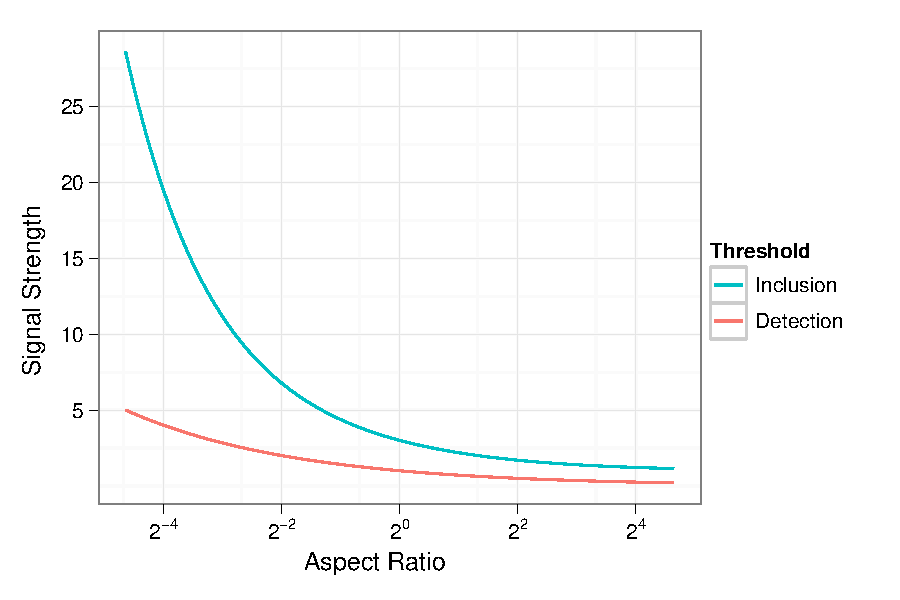
\includegraphics{frobenius-loss-cutoff}
    \caption{
        \captiontitle{Signal Strength Thresholds}
        Detection threshold $\gamma^{-1/2}$ and
        inclusion threshold
        \(
            \mu_\Frob^\ast
            =
            \frac{1 + \gamma^{-1}}{2}
            +
            \sqrt{
                \left( \frac{1 + \gamma^{-1} }{2} \right)^2
                +
                \frac{3}{\gamma}
            }
        \)
        plotted against the aspect ratio $\gamma = \frac{n}{p}$.  When
        the normalized signal strength $\frac{\mu_i}{\sigma^2}$ is above the 
        detection threshold, the $i$th sample SVD factors are correlated with
        the population factors.  With respect to Frobenius loss, when the 
        normalized signal strength is above the inclusion threshold, it is 
        beneficial to include the $i$th term in the SVD approximation of 
        $\sqrt{n} \, \mU_n \mD_n \mV_n^\trans$.
    }\label{F:frobenius-loss-cutoff}
\end{figure}

\clearpage

\section{Simulations}\label{S:intrinsic-loss-simulations}

We confirm the theory of the previous section with a Monte Carlo simulation.  We generate a matrix $\mX$ as follows:
\begin{enumerate}
    \item The concentration $\gamma$ is one of $\{ 0.25, 1.0, 4.0 \}$.
    \item The size of the matrix $s$ is one of $\{ 144, 400, 1600, 4900 \}$.
        We set the number of rows and columns in the matrix as
        $n = \sqrt{ s \, \gamma }$ and $p = \sqrt{s / \gamma}$, respectively.
        This ensures that $\gamma = \frac{n}{p}$ and $s = n \, p$.
    \item The noise level is set at $\sigma^2 = 1$.  The noise matrix $\mE$
        is an $n \times p$ matrix with \iid $\Normal\left( 0, \, 1\right)$
        elements.
    \item The generative rank, $k_0$, is fixed at $5$.  The normalized
        factor strengths are set at
        \(
            (
                \mu_1, \,
                \mu_2, \,
                \mu_3, \,
                \mu_4, \,
                \mu_5
            )
            =
            (
                4 \mu_\Frob^\ast, \,
                2 \mu_\Frob^\ast, \,
                  \mu_\Frob^\ast, \,
                \frac{1}{2} \mu_\Frob^\ast, \,
                \frac{1}{4} \mu_\Frob^\ast
            ),
        \)
        and the factor strength matrix is
        \(
            \mD 
            = 
            \diag\left( 
                \mu_1^{1/2},
                \mu_2^{1/2},
                \ldots, 
                \mu_5^{1/2}
            \right).
        \)
    \item The left and right factor matrices $\mU$ and $\mV$ are of sizes
        $n \times 5$ and $p \times 5$, respectively.  We choose these matrices
        uniformly at random over the Stiefel manifold according
        to Algorithm~\ref{A:random-steifel} in Appendix~\ref{A:projections}.
    \item We set $\mX = \sqrt{n} \, \mU \mD \mV^\trans + \mE$ and let
        $\mhX(k)$ be the SVD of $\mX$ truncated to $k$ terms.
\end{enumerate}
After generating $\mX$, we compute the squared Frobenius loss
\(
    \frac{1}{n} \| \sqrt{n}\mU \mD \mV^\trans - \mhX(k) \|_F^2
\)
and the squared spectral loss
\(
    \frac{1}{n} \| \sqrt{n}\mU \mD \mV^\trans - \mhX(k) \|_2^2
\)
as functions of the rank, $k$.  In 
Figures~\ref{F:frob2-loss-sim}~and~\ref{F:spec2-loss-sim}, we plot the results 
over 500 replicates.  For the Frobenius case, we should expect the loss to
decrease until $k=2$, stay flat at $k=3$, and then increase thereafter.  This 
is confirmed by the simulations.  The spectral norm behaves similarly to the 
Frobenius norm.


\begin{figure}[tbh]
    \centering
    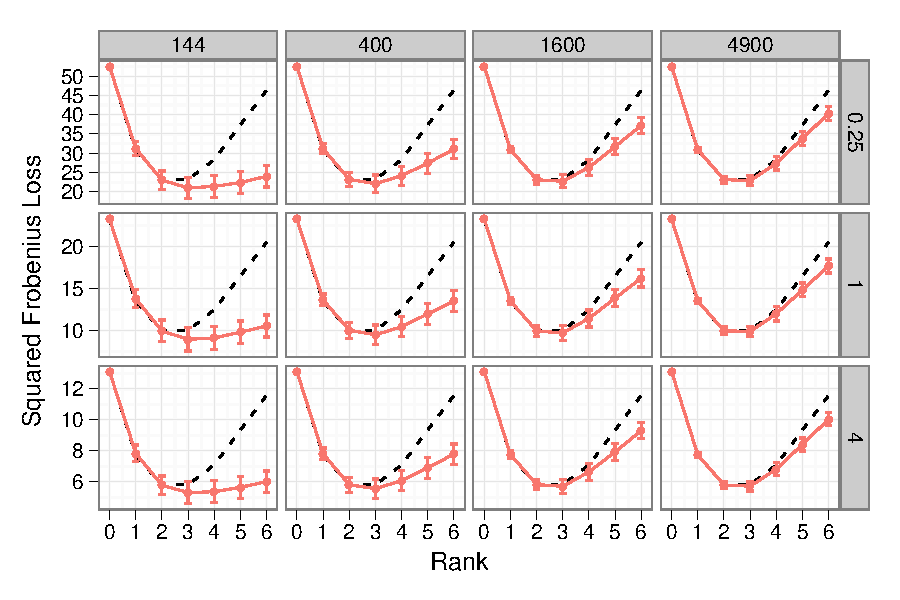
\includegraphics{frob2-loss-sim}
    \caption{
        \captiontitle{Frobenius Loss Penalty}
        Squared Frobenius loss
        \(
            \frac{1}{n} \| \sqrt{n}\mU \mD \mV^\trans - \mhX(k) \|_F^2
        \)
        as a function of the rank, $k$, for
        $\mX$ generated according the the procedure described
        in Section~\ref{S:intrinsic-loss-simulations} and $\mhX(k)$ equal
        to the SVD of $\mX$ truncated to $k$ terms.  The concentration 
        $\gamma = \frac{n}{p}$ is one of $\{ 0.25, 1.0, 4.0 \}$ and the
        size $s = n p$ is one of $\{ 144, 400, 1600, 4900 \}$.  
        The solid lines show the means over $500$ replicates with the error 
        bars showing one standard deviation.  The dashed lines show the 
        predictions from Section~\ref{S:loss-behavior}.  We can see that as 
        the size increases, the simulation agrees more and more with the 
        theory.
    }\label{F:frob2-loss-sim}
\end{figure}

\begin{figure}[hbt]
    \centering
    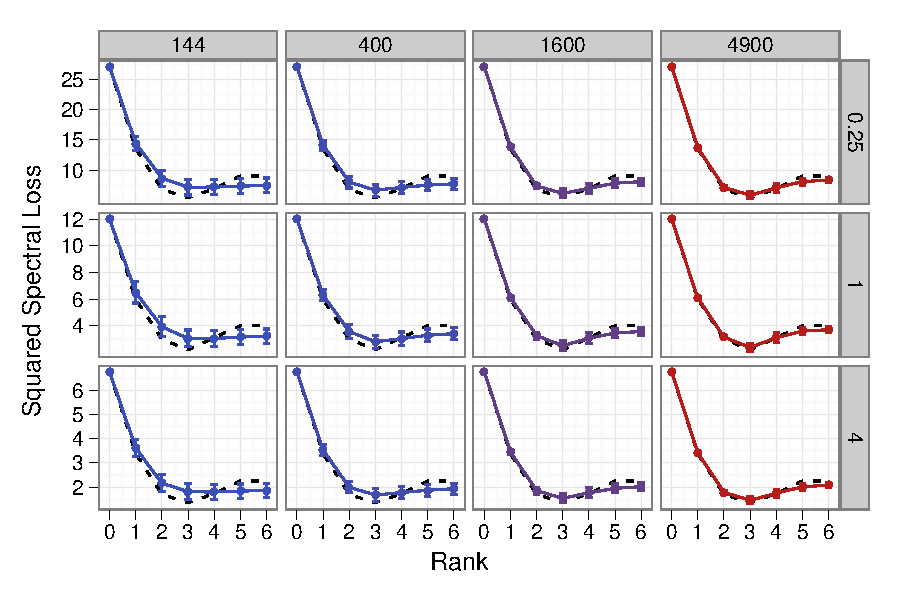
\includegraphics{spec2-loss-sim}
    \caption{
        \captiontitle{Spectral Loss Penalty}
        Squared spectral loss
        \(
            \frac{1}{n} \| \sqrt{n}\mU \mD \mV^\trans - \mhX(k) \|_2^2
        \)
        as a function of the rank, $k$, with $\mX$ and $\mhX(k)$ as in
        Figure~\ref{F:frob2-loss-sim}.  Sample size $s = n p$ is shown in the 
        columns and concentration $\gamma = \frac{n}{p}$ is shown in the rows.
        Solid lines show the means
        over $500$ replicates with the error bars showing one standard 
        deviation; the dashed lines show the predictions from 
        Section~\ref{S:loss-behavior}.  The simulations agrees quite well
        with the theory, especially for large sample sizes.
    }\label{F:spec2-loss-sim}
\end{figure}

\clearpage

\section{Relation to the scree plot}\label{S:intrinsic-rank-scree-plot}

Cattell's scree plot~\cite{cattell1966scree} is a popular device for choosing
the truncation rank in principal components analysis. One plots the square of
the singular value, $\hat d^2_k$, against the component number, $k$. Typically
such a plot exhibits an ``elbow'', where the slope changes noticeably. This is
the point at which Cattell recommends truncating the SVD of the matrix.

In some circumstances, the elbow is close to the Frobenius and spectral loss
minimizers, $k_\Frob^\ast$ and $k_2^\ast$. In Figure~\ref{F:scree-elbow}, we
generate a matrix
\(
    \mX = \sqrt{n} \, \mU \mD \mV^\trans + \mE \in \reals^{n \times p},
\)
with $n = p = 100$, such that elements of $\mE$ are \iid $\Normal( 0, \, 1)$. 
In the first column, we set
\(
    \mD^2 = \diag( 5.0, \, 4.75, \, 4.5, \, \ldots, \, 0.5, \, 0.25 ).
\)
The figure shows the scree plot along with
\(
    \| \sqrt{n} \, \mU \mD \mV^\trans - \mhX(k) \|^2
\) 
for Frobenius and spectral norms, where $\mhX(k)$ is the SVD of $\mX$
truncated to $k$ terms. There is substantial ambiguity in determining the
location of the most pronounced elbow. Despite this subtlety, there is indeed 
an elbow relatively close to $k_\Frob^\ast$ and $k_2^\ast$, the minimizers of 
the two loss functions.

We can easily manipulate the simulation to get a scree plot with a more 
pronounced elbow in the wrong place.  In the second column of Figure~\ref{F:scree-elbow}, we augment the factor strength matrix with three additional large values, so that
\(
    \mD^2 
    = 
    \diag( 
        20.0, \, 15.0, \, 10.0, \,
        5.0, \, 4.75, \, 4.5, \, \ldots, \, 0.5, \, 0.25 
    ).
\)
With this modification, there is a clear elbow at $k=4$.  However, compared to 
the optimal values, truncating the SVD at $k=4$ gives about a 25\% worse error 
with respect to squared Frobenius loss and about 50\% worse with respect to 
squared spectral loss.

In general, we cannot make any assurances about how close the elbow is to 
$k_\Frob^\ast$ or $k_2^\ast$.  Through a simulation study, 
Jackson~\cite{jackson1993stopping} provides evidence that if the latent 
factors are strong enough to be easily distinguished from noise, then the 
elbow is a reasonable estimate of the loss minimizers (he does not actually compute the loss behavior, but this seems likely).  However, when there 
are both well-separated factors and factors near the critical strength level 
$\mu_\Frob^\ast$, the second example here illustrates that the elbow might be 
a poor estimate.

\begin{figure}[ht]
    \begin{center}
        \begin{minipage}{0.49\textwidth}
            \begin{center}
                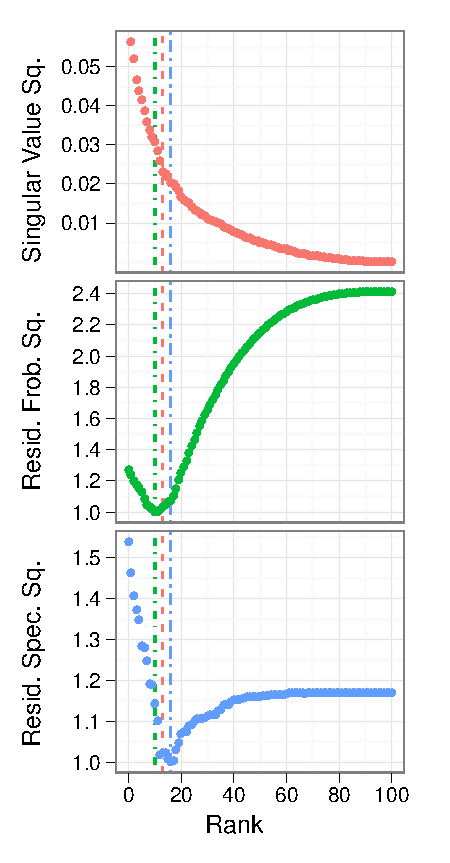
\includegraphics{scree-elbow-right}
            \end{center}
        \end{minipage}
        \begin{minipage}{0.49\textwidth}
            \begin{center}
                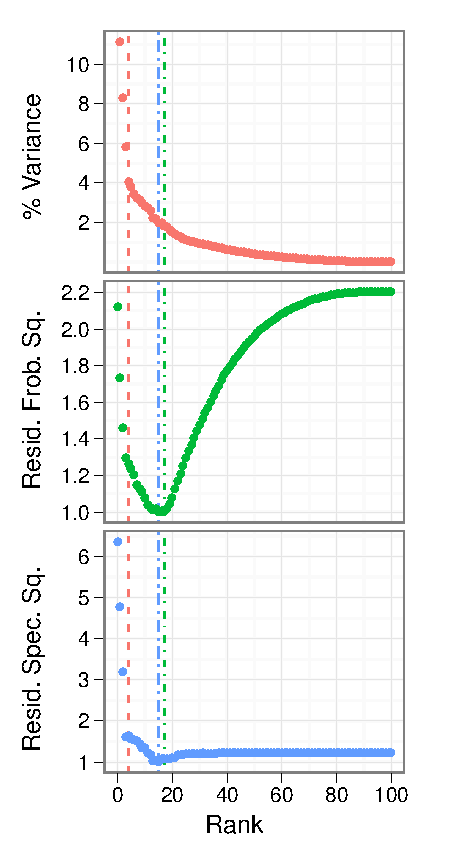
\includegraphics{scree-elbow-left}
            \end{center}
        \end{minipage}
        \caption{
            \captiontitle{Scree Plots and Loss Functions}
            We generate a matrix as 
            $\mX = \sqrt{n} \, \mU \mD \mV^\trans + \mE$ 
            and set $\mhX(k)$ equal to the SVD of $\mX$ truncated to $k$ 
            terms.  The left and right columns show different choices of
            $\mD$, described in the text.  The top row contains scree plots, 
            where the square of the $k$th singular value of $\mX$,
            $\hat d_k^2$, is plotted against 
            component number, $k$, with units are chosen so that 
            $\sum_{k} \hat d_k^2 = 1$.  The next two rows show
            $\| \sqrt{n} \, \mU \mD \mV^\trans - \mhX(k) \|_\Frob^2$ and
            $\| \sqrt{n} \, \mU \mD \mV^\trans - \mhX(k) \|_2^2$, as functions
            of the rank, $k$ with units chosen so that the minimum value is
            $1.0$.  Dashed lines show the elbow of the scree plot and the
            minimizers of the two loss functions.  
            The elbow of the scree plot gives a reasonable estimate of
            the loss minimizers in the first column, but not in the second.
        }\label{F:scree-elbow}
    \end{center}
\end{figure}

\clearpage

\section{Extensions}\label{S:intrinsic-rank-extensions}

We have focused specifically on truncating the singular value decomposition
because that is the case for which the theory has been most developed. We have
also focused specifically on Frobenius and spectral losses. One could easily
extend our work to look at the nuclear norm loss (sum of singular values)
\cite{fazel2002mrm} or Stein's loss \cite{james1961ewq}. Alternatively, it is
not hard to adapt our analysis to study forms like $\| \mhU \mhD(k)^2
\mhU^\trans - \mU \mD^2 \mU^\trans \|$. For matrix decompositions beyond the
SVD, extension of our work is more difficult, mainly because very little
scholarship has been devoted to their theoretical properties.

We have not examined shrinking the singular values at all, but in some 
situations this may be beneficial.  For example, the Frobenius norm of the $\mF_i$ matrix from Section~\ref{S:loss-behavior}, which is involved in the Frobenius loss
\(
    \| \sqrt{n} \, \mU \mD \mV^\trans - \mhX(k) \|_F^2,
\)
converges to
\[
    \mu_i - 2 \varphi_i \theta_i \mu_i^{1/2} \bmu_i^{1/2} + \bmu_i
\]
whenever $k \geq i$.  Recall that $\bmu_i$ is the almost-sure limit of
the $\hat d_i^2$, the square of the $i$th singular value of $\frac{1}{\sqrt{n}} \mX$.  If we shrink the $i$th singular value, replacing
$\hat d_i$ with $f(\hat d_i)$ for continuous $f(\cdot)$, then the Frobenius penalty for including the $i$th term converges to
\[
    \mu_i 
    - 2 \varphi_i \theta_i \mu_i^{1/2} f( \bmu_i^{1/2} ) 
    + f^2( \bmu_i^{1/2} ).
\]
This quantity is minimized when
\(
    f( \bmu_i^{1/2}) 
        = \mu_i^{1/2} \varphi_i \theta_i
        = \bmu_i^{-1/2} 
          \left( \mu_i - \frac{\sigma^4}{ \gamma \mu_i } \right).               
\)
After some algebra, the optimal $f$ takes the form
\[
    f( \hat d_i )
        =
        \begin{cases}
        \left(
            \hat d_i^2
            -
            2
            \big(
                1 + \frac{1}{\gamma}
            \big)
            \sigma^2
            +
            \big(
                1 - \frac{1}{\gamma}
            \big)^2
            \frac{\sigma^4}
                 {\hat d_i^2}
        \right)^{1/2}
            &\text{when $\hat d_i 
                         > 
                         \sigma 
                         \left(
                            1 + \frac{1}{\sqrt{\gamma}}
                         \right)$,} \\
        0 
            &\text{otherwise.}
        \end{cases}
\]
With this shrinkage, it is always beneficial (in terms of Frobenius norm) to include the $i$th term.
